% Generated by `uv run python -m gainpred.writeup`; do not edit by hand.
\begin{figure}[htbp]
\centering
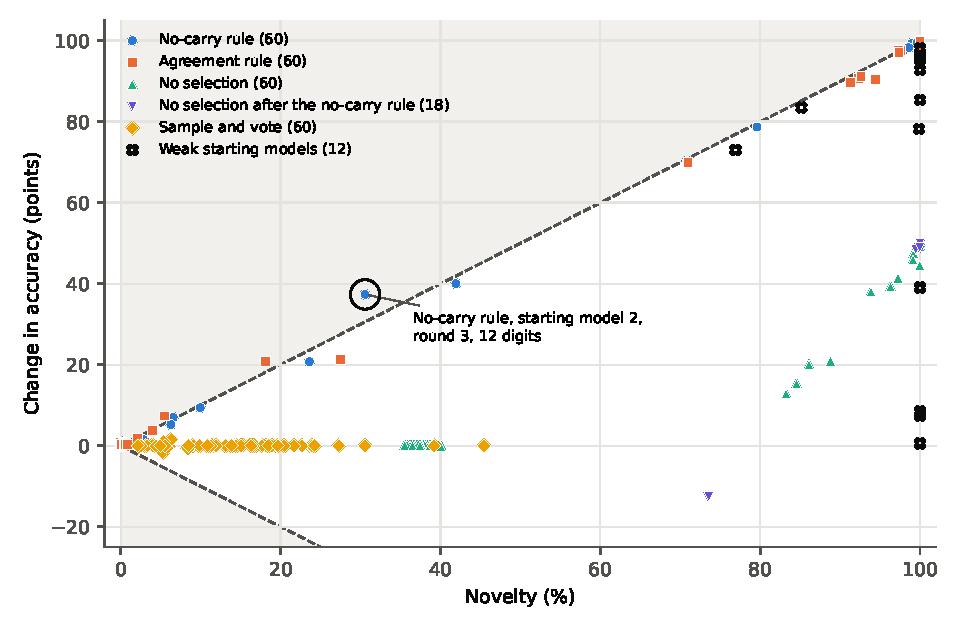
\includegraphics[width=\linewidth]{generated/figure_novelty_gain.pdf}
\caption{Change in accuracy against novelty, one point per evaluation case (all
  270, with or without an outcome); computed after the evaluation runs. Novelty
  is measured on the teacher's kept answers before the round; accuracy on the
  test problems of that length, after the round minus before (points). Dashed:
  change = novelty and change = minus novelty, the bound a teacher's novelty
  sets on how far it can move the student; shaded: outside it. Circled: the one
  case more than 3 points outside.}
\label{fig:novelty-gain}
\end{figure}
